\section{Lecture 27}
\subsection{Lecture Notes - Scattering Theory}
\subsubsection{Motivation}
Scattering Theory is very useful for probing information on atomic scales, in condensed matter/nuclear/atomic physics. A familiar example is Rutherford scattering:
\begin{center}
    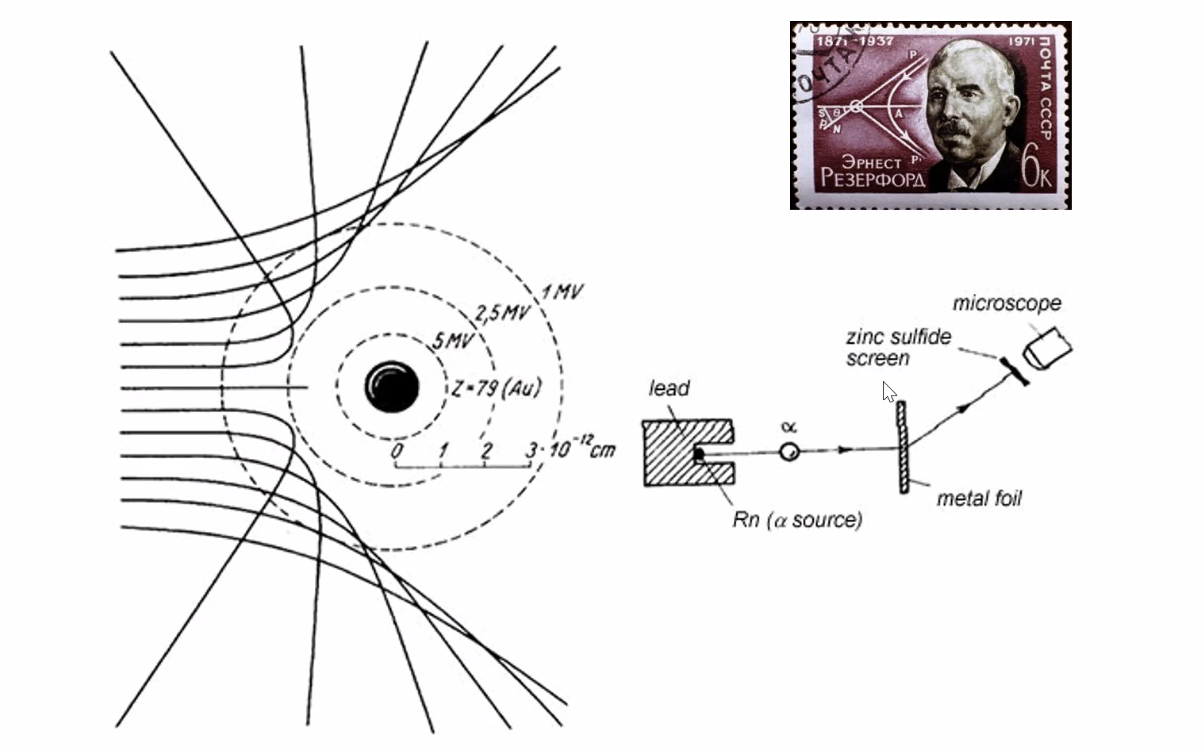
\includegraphics[scale=0.5]{Lecture-27/l27-img1.png}
    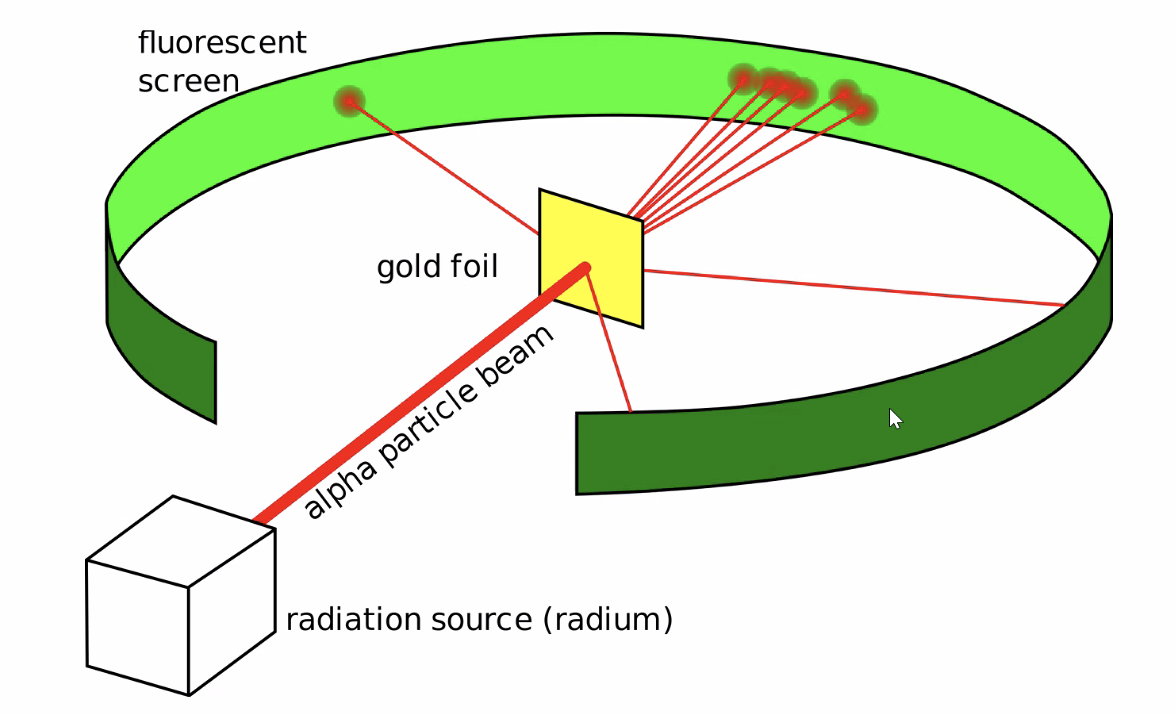
\includegraphics[scale=0.5]{Lecture-27/l27-img2.png}
\end{center}
Where $\alpha$ particles (Helium nuclei) were scattered off of gold atoms, and large deflections were observed.

\subsubsection{Fundamental parameters}
There are a couple quantities that are of relevance to consider. First, we have the impact parameter $b$, which is the perpendicular distance from the incoming trajectory to the parallel axis through the center of the target. Then, we have the scattering angle $\theta$, which is the angle between the initial and final velocities. The simplest possible interaction is the hard-sphere interaction:
\begin{center}
    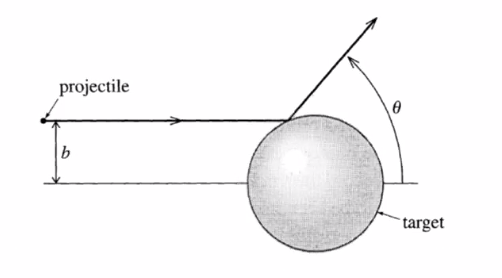
\includegraphics[scale=0.8]{Lecture-27/l27-img3.png}
\end{center}
Now, lets consider a beam of area $A$ passing through a target of length $L$ and number density of particles $n$. Assume the target is larger in the cross sectional area than in the beam. What is the total number of target particles in the beam?
\begin{center}
    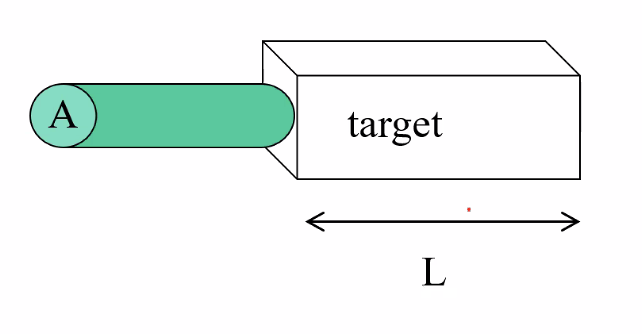
\includegraphics[scale=0.7]{Lecture-27/l27-img4.png}
\end{center}
\begin{s}
Since $n$ gives the volume number density, we have that $AL$ gives the volume of the beam in the target and hence the total number of target particles is given by $nAL$.
\end{s}
Next, the \textbf{cross-section} $\sigma$ is defined as the effective area of target for interacting with the particle. For hard spheres of radius $R$, we have that $\sigma = \pi R^2$ (the cross-sectional area of a circle). 
\begin{center}
    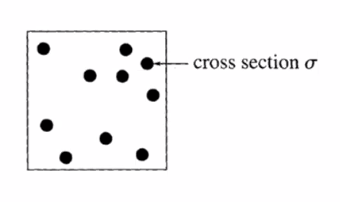
\includegraphics[scale=0.8]{Lecture-27/l27-img5.png}
\end{center}
Now, given this cross section $\sigma$ of a single target particle, what is the probability that any one projectile makes a hit (assume the same scenario above with the beam of area $A$, the target of length $L$?)
\begin{s}
By dimensional analysis, since probability is dimensionless, since $n$ has units of inverse volume, then $L$ has units of length and $\sigma$ has units of area and hence this works out. This makes sense as the probability should scale with the cross-sectional area of a target particle, the length of the target, and the number density of the target. A way to see that the area $A$ of the beam drops out to see is that:
\[P(\text{hit}) = \frac{\text{Area of all targets}}{A} = \frac{n\sigma A L}{A} = n\sigma L\]
\end{s}
Given the beam has an incident rate $R_{inc}$ of incoming particles per unit time, what is the scattered rate (number of scattered particles per unit time?)
\begin{s}
The rate would just be $R_{inc}\sigma n L$, just multiply the scattering probability by the incoming rate.
\end{s}

\subsubsection{Example: Scattering Neutrons on Aluminum Foil}
Take $N_{\text{inc}} = 10000$. the alumnimum foil has thickness of $0.1\text{mm}$. For neutrons, we have that $\sigma = 1.5 \cdot 10^{-28}\text{m}^2$. Since this is such a common unit in nuclear physics, this is often denoted with a new unit, the \textit{barn} ($1 \text{barn} = 1\times 10^{-28}\text{m}^2$; i.e. $\sigma = 1.5\text{barns}$. For alumnimum, we have mass density $\rho_{Al} = 2.7\times 10^3 \text{kg/m}^3$ and we know that $m_{Al} = 27u$. Hence, the scattered number of particles is given by:
\[N_{\text{scatter}} = N_{\text{inc}}\frac{\rho_{\text{Al}}}{m_{Al}}L\sigma = 9\]


\subsubsection{Example: Scattering of Two Hard Spheres}
In this case, we have effective scattering area of $\pi(R_1 + R_2)^2$.
\begin{center}
    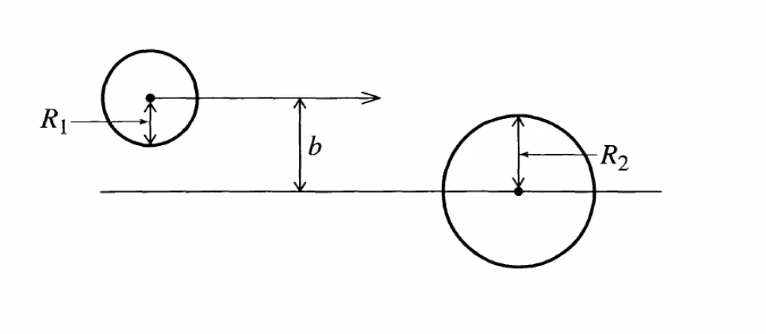
\includegraphics[scale=0.7]{Lecture-27/l27-img6.png}
\end{center}

\subsubsection{Example: Mean free path of air molecule}
Air molecules can be approximated as hard spheres with $R = 0.15\text{nm}$. Define the quantity \textbf{mean free path} $\lambda$ as the average distance between two collisions. For sigma, we take (from the formula above):
\[\sigma = \pi(2R)^2 = 4\pi R^2\]
We have number density:
\[n = \frac{N}{V}\]
The probability of a collision when travelling a distance $dx$ is given by:
\[P(\text{coll in dx}) = n\sigma dx\]
Hence the probability of having a first collision in $x$ and $x + dx$ as:
\[P(\text{first coll between in x and x + dx}) = P(\text{no coll in x})\cdot n \sigma dx\]
We can write this in another way as:
\[P(\text{first coll between in x and x + dx}) = P(\text{no coll in x}) - P(\text{no coll in x + dx})\]
Turning this small $dx$ into a differential, we have:
\[P(\text{first coll between in x and x + dx}) = -\dod{}{x}P(\text{no coll in x})\]
We call $P(\text{no coll in x})$ as $P(x)$ for notations. Setting the two expressions equal to each other, we have:
\[\dod{}{x}P(x) = -\frac{N\sigma}{V}P(x)\]
This has solution:
\[P(x) = \exp(-\frac{N\sigma}{V}x)\]
Then the mean free path can be calculated as the average value of x given this probaility distribution:
\[\lambda = \avg{x} = \int_{0}^{\infty}xP(x)dx = \int_0^\infty xn\sigma \exp(-\frac{N\sigma}{V}x)\]
Note that the $n\sigma$ is there as a normalization factor for the distribution. Taking this integral, we have:
\[\lambda = \frac{1}{n\sigma}\]
This makes sense intuitively; the larger the cross section and the larger the number density, the smaller the mean free path between collisions. Dimensionally, this also has units of length, which is good! At STP, we can calculate what this would be numerically:
\[\lambda = \frac{V_a}{N_a(4\pi R^2)} \approx 130\text{nm}\]

\subsubsection{Solid Angle}
\begin{center}
    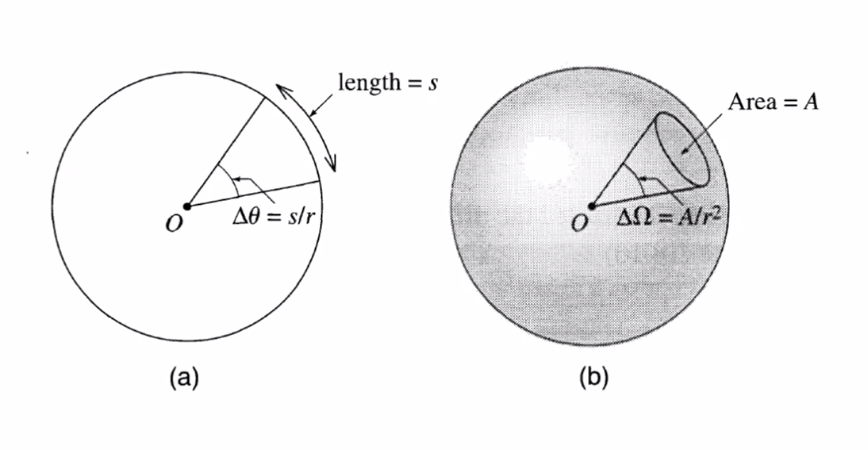
\includegraphics[scale=0.5]{Lecture-27/l27-img7.png}
\end{center}
We are familiar with the normal angle, $\Delta \theta = \frac{s}{r}$, the ratio of the arc length to the radius. Generalizing this to 3D, we have the solid angle, $\Delta \Omega = \frac{A}{r^2}$ where $A$ is the "arc area" and $r$ the radius. For a cone with polar angles $\theta, \theta + d\theta$, $\phi, \phi + d\phi$. The expression is therefore given by:
\[d\Omega = \sin\theta d\theta d\phi\]
What is the integral of the solid angle increment $d\Omega$ over all possible solid angles (over the surface of a sphere?)
\begin{s}
$\int d\Omega = 4\pi$ (surface area of unit sphere). We could actually do the integral, or we could just recognize that the surface area of a sphere is given as $4\pi r^2$ and divide this by $r^2$. 
\end{s}

\subsubsection{Differential Cross Section}
Typical scenario is we have that a detector covers some portion of a sphere around our target.
\begin{center}
    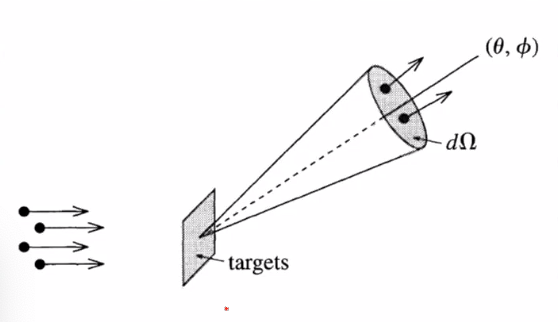
\includegraphics[scale=0.8]{Lecture-27/l27-img8.png}
\end{center}
We must have that:
\[N_{\text{scatter}}(\text{into d$\Omega$}) = N_{inc}n_{target}d\sigma(\text{into d$\Omega$}) = N_{inc}n_{target}\left(\dod{\sigma}{\Omega}(\theta, \phi)\right)d\Omega\]
The term $\od{\sigma}{\Omega}(\theta, \phi)$ is the differential cross section. This can be measured in experiment, or predicted in theory. We can also obtain the total cross section, which is the integral over all differnetial cross sections.
\[\sigma_{tot} = \int \dod{\sigma}{\Omega}(\theta, \phi) d\Omega = \int_0^\pi \sin\theta d\theta \int
_0^{2\pi}d\phi\dod{\sigma}{\Omega}\]
For a beam with area $A$ and total number of particles $N$, what is the total number of particles $dN$ that passes through the segment between $b$ and $b + db$ and $\phi$ and $\phi + d\phi$?
\begin{center}
    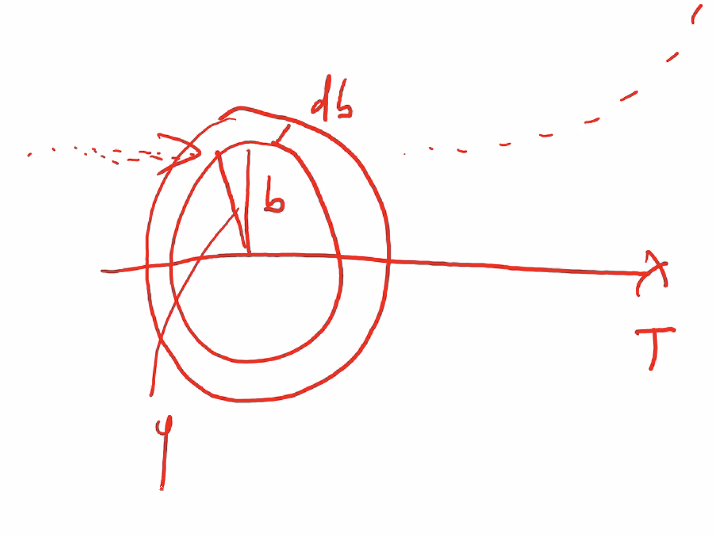
\includegraphics[scale=0.7]{Lecture-27/l27-img9.png}
\end{center}
\begin{s}
We know that the area of the segment is given by $b dbd\phi$, and then dividing this by the total area $A$ we get the fraction of particles that would hit that area. Hence, $dN = \frac{N}{A}bdbd\phi$.
\end{s}
Note that for the case with axial symmetry, we have:
\begin{center}
    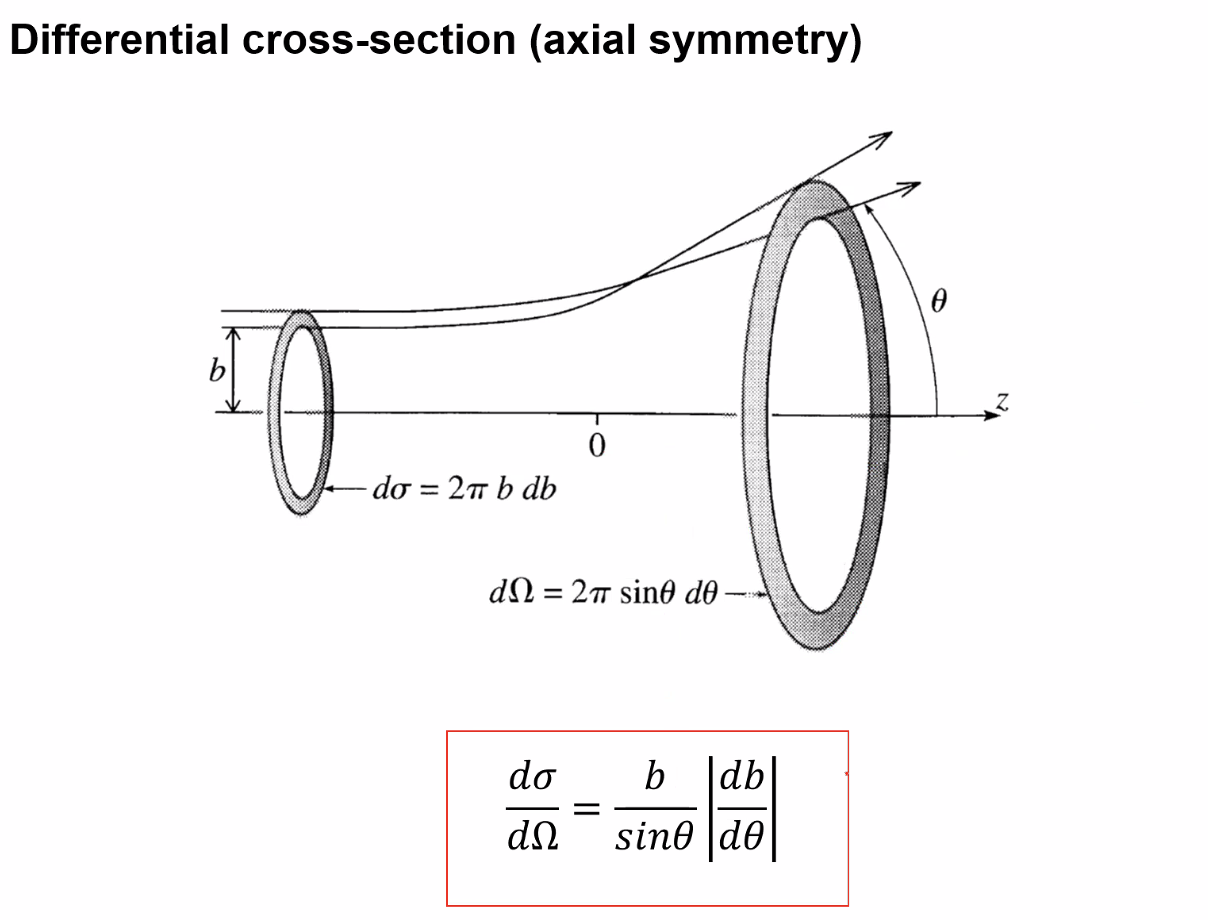
\includegraphics[scale=0.7]{Lecture-27/l27-img10.png}
\end{center}
But we will continue this discussion next day.